\section{IOT}
\subsection{Pengertian IoT}
\textbf{Internet of Things (IoT)} adalah konsep di mana benda-benda fisik sehari-hari dilengkapi dengan kemampuan untuk mengumpulkan, memproses, dan bertukar data melalui jaringan, tanpa memerlukan interaksi manusia secara langsung (\textit{machine-to-machine} / M2M). 

Inti dari IoT adalah menjembatani dunia fisik (\textit{physical world}) dan dunia digital (\textit{cyber world}) sehingga benda mati bisa "berpikir" sederhana, dan "bertindak".

Tujuan utama dari IoT adalah menciptakan lingkungan yang lebih cerdas (\textit{smart environment}), efisien, dan otomatis, di mana data yang dikumpulkan oleh perangkat dapat dianalisis untuk menghasilkan wawasan (\textit{insight}) yang bermanfaat, mendukung pengambilan keputusan, serta meningkatkan kenyamanan dan produktivitas manusia.

\subsubsection{Karakteristik Utama IoT}
\begin{itemize}
    \item \textbf{Konektivitas (\textit{Connectivity}):} Perangkat mampu terhubung ke internet atau jaringan lokal.
    \item \textbf{Sensing:} Memiliki sensor untuk mendeteksi kondisi lingkungan sekitar.
    \item \textbf{Otomatisasi (\textit{Automation}):} Dapat bekerja dan mengambil tindakan tanpa campur tangan manusia secara langsung.
    \item \textbf{Pertukaran Data (\textit{Data Exchange}):} Mampu mengirim dan menerima data secara \textit{real-time}.
    \item \textbf{Interoperabilitas:} Dapat berkomunikasi dengan berbagai jenis perangkat dan platform yang berbeda.
\end{itemize}

\subsection{Sejarah IoT}
Berikut adalah garis waktu (\textit{timeline}) perkembangan konsep dan teknologi Internet of Things dari masa ke masa:

\begin{center}
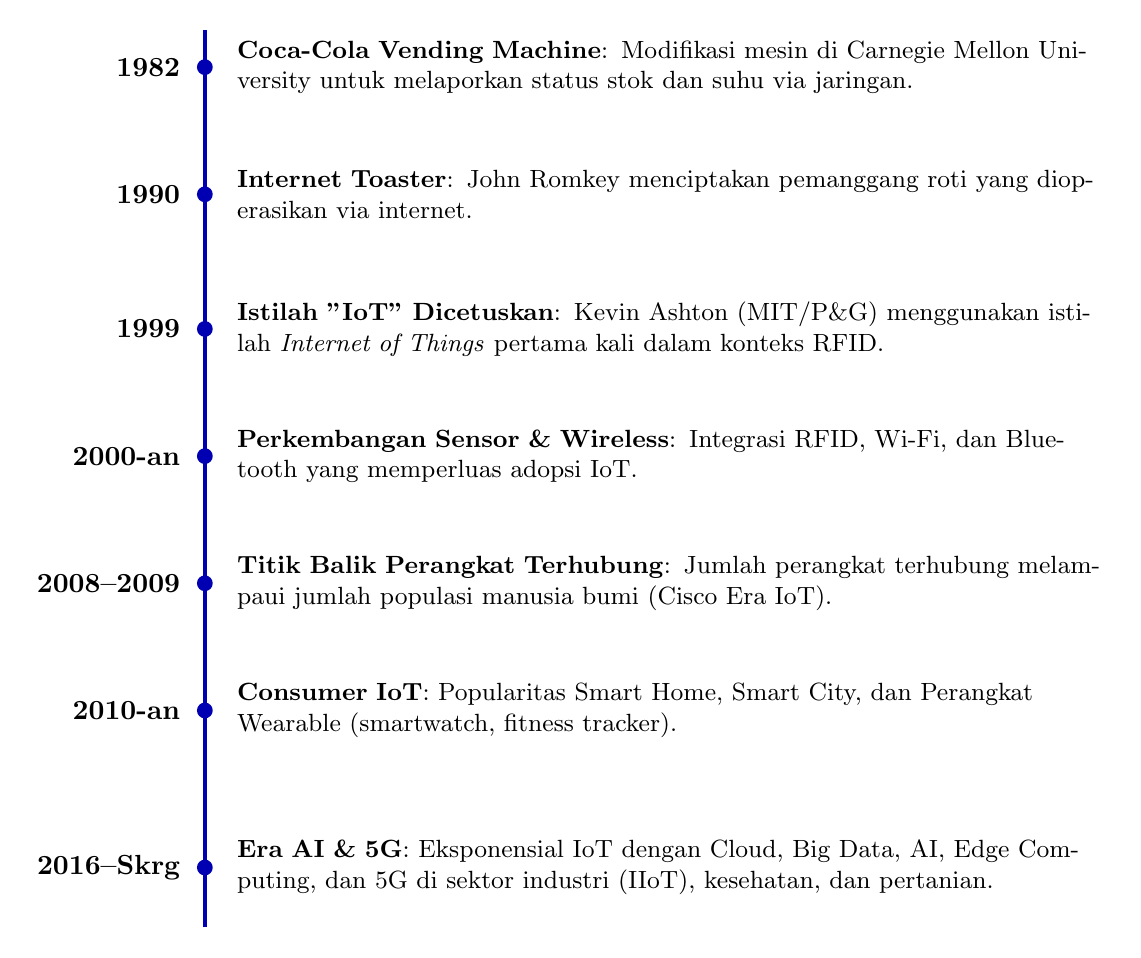
\begin{tikzpicture}[scale=0.95, every node/.style={font=\small}]
    % Garis Utama Timeline
    \draw[line width=1.5pt, color=blue!70!black] (0,0) -- (0,12);
    
    % 1982
    \fill[blue!70!black] (0,11.5) circle (3pt);
    \node[anchor=east, font=\bfseries] at (-0.2, 11.5) {1982};
    \node[anchor=west, text width=11cm] at (0.3, 11.5) {\textbf{Coca-Cola Vending Machine}: Modifikasi mesin di Carnegie Mellon University untuk melaporkan status stok dan suhu via jaringan.};
    
    % 1990
    \fill[blue!70!black] (0,9.8) circle (3pt);
    \node[anchor=east, font=\bfseries] at (-0.2, 9.8) {1990};
    \node[anchor=west, text width=11cm] at (0.3, 9.8) {\textbf{Internet Toaster}: John Romkey menciptakan pemanggang roti yang dioperasikan via internet.};
    
    % 1999
    \fill[blue!70!black] (0,8.0) circle (3pt);
    \node[anchor=east, font=\bfseries] at (-0.2, 8.0) {1999};
    \node[anchor=west, text width=11cm] at (0.3, 8.0) {\textbf{Istilah "IoT" Dicetuskan}: Kevin Ashton (MIT/P\&G) menggunakan istilah \textit{Internet of Things} pertama kali dalam konteks RFID.};
    
    % 2000-an
    \fill[blue!70!black] (0,6.3) circle (3pt);
    \node[anchor=east, font=\bfseries] at (-0.2, 6.3) {2000-an};
    \node[anchor=west, text width=11cm] at (0.3, 6.3) {\textbf{Perkembangan Sensor \& Wireless}: Integrasi RFID, Wi-Fi, dan Bluetooth yang memperluas adopsi IoT.};
    
    % 2008-2009
    \fill[blue!70!black] (0,4.6) circle (3pt);
    \node[anchor=east, font=\bfseries] at (-0.2, 4.6) {2008--2009};
    \node[anchor=west, text width=11cm] at (0.3, 4.6) {\textbf{Titik Balik Perangkat Terhubung}: Jumlah perangkat terhubung melampaui jumlah populasi manusia bumi (Cisco Era IoT).};
    
    % 2010-an
    \fill[blue!70!black] (0,2.9) circle (3pt);
    \node[anchor=east, font=\bfseries] at (-0.2, 2.9) {2010-an};
    \node[anchor=west, text width=11cm] at (0.3, 2.9) {\textbf{Consumer IoT}: Popularitas Smart Home, Smart City, dan Perangkat Wearable (smartwatch, fitness tracker).};
    
    % 2016-Sekarang
    \fill[blue!70!black] (0,0.8) circle (3pt);
    \node[anchor=east, font=\bfseries] at (-0.2, 0.8) {2016--Skrg};
    \node[anchor=west, text width=11cm] at (0.3, 0.8) {\textbf{Era AI \& 5G}: Eksponensial IoT dengan Cloud, Big Data, AI, Edge Computing, dan 5G di sektor industri (IIoT), kesehatan, dan pertanian.};
\end{tikzpicture}
\end{center}

\subsection{Arsitektur IoT}
Arsitektur sistem IoT umumnya dibagi menjadi 4 lapisan (\textit{layers}) utama:

\begin{center}
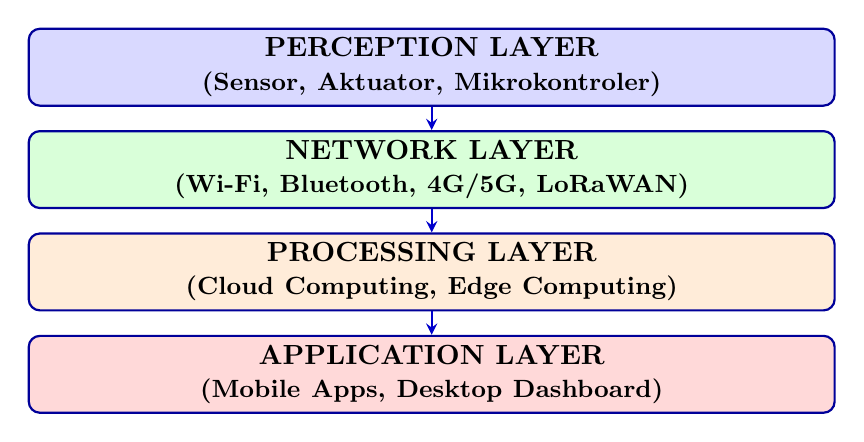
\begin{tikzpicture}[node distance=1.3cm, auto,
    layer/.style={draw=blue!60!black, thick, fill=blue!10, text width=10cm, align=center, rounded corners=4pt, minimum height=0.9cm, font=\bfseries},
    arrow/.style={->, >=stealth, thick, color=blue!80!black}]
    
    \node (perc) [layer, fill=blue!15] {PERCEPTION LAYER \\ \small(Sensor, Aktuator, Mikrokontroler)};
    \node (net) [layer, fill=green!15, below of=perc] {NETWORK LAYER \\ \small(Wi-Fi, Bluetooth, 4G/5G, LoRaWAN)};
    \node (proc) [layer, fill=orange!15, below of=net] {PROCESSING LAYER \\ \small(Cloud Computing, Edge Computing)};
    \node (app) [layer, fill=red!15, below of=proc] {APPLICATION LAYER \\ \small(Mobile Apps, Desktop Dashboard)};
    
    \draw [arrow] (perc) -- (net);
    \draw [arrow] (net) -- (proc);
    \draw [arrow] (proc) -- (app);
\end{tikzpicture}
\end{center}

\begin{description}
    \item[Perception Layer:] Lapisan fisik atau perangkat keras paling dasar yang bertugas mengumpulkan data dari lingkungan nyata (seperti panca indra manusia). Mengubah kondisi fisik menjadi data digital. \textit{Contoh: Sensor, Aktuator, Mikrokontroler.}
    \item[Network Layer:] Lapisan infrastruktur konektivitas yang merutekan dan mentransmisikan data dari perception layer menuju server cloud atau pusat data. \textit{Contoh: Wi-Fi, Bluetooth, GSM/4G/5G, LoRaWAN.}
    \item[Processing Layer:] Lapisan "otak" sistem yang menyaring, menganalisis, dan mengolah data mentah menjadi informasi bermakna memanfaatkan teknologi \textit{Cloud Computing} atau \textit{Edge Computing}.
    \item[Application Layer:] Lapisan teratas yang berfungsi sebagai antarmuka langsung (\textit{User Interface}) bagi pengguna untuk memantau dan mengendalikan perangkat pintar secara \textit{real-time}.
\end{description}

\subsection{Cara Kerja IoT}
Secara umum, alur kerja sistem IoT terbagi menjadi empat langkah berurutan:

\begin{center}
\begin{tikzpicture}[node distance=1.3cm, auto,
    layer/.style={draw=blue!60!black, thick, fill=blue!10, text width=10cm, align=center, rounded corners=4pt, minimum height=0.9cm, font=\bfseries},
    arrow/.style={->, >=stealth, thick, color=blue!80!black}]
    
    \node (sens) [layer, fill=blue!15] {SENSING};
    \node (conn) [layer, fill=green!15, below of=perc] {CONNECTING};
    \node (proc) [layer, fill=orange!15, below of=net] {PROCESSING};
    \node (act) [layer, fill=red!15, below of=proc] {ACTING};
    
    \draw [arrow] (sens) -- (conn);
    \draw [arrow] (conn) -- (proc);
    \draw [arrow] (proc) -- (act);
\end{tikzpicture}
\end{center}

\begin{enumerate}
    \item \textbf{Sensing:} Sensor mendeteksi kondisi fisik lingkungan (suhu, kelembapan, cahaya, gerakan, posisi) dan mengubahnya menjadi sinyal digital.
    \item \textbf{Connecting:} Data dikirimkan melalui jaringan komunikasi (Wi-Fi, Bluetooth, Seluler, MQTT) menuju gateway atau server.
    \item \textbf{Processing:} Data diolah dan dianalisis pada cloud/edge computing untuk menghasilkan wawasan atau perintah.
    \item \textbf{Acting:} Sistem memberikan notifikasi kepada pengguna atau menginstruksikan akuator secara otomatis untuk melakukan tindakan fisik.
\end{enumerate}

\subsection{Komponen Utama IoT}
Sistem IoT dibangun dari beberapa komponen kunci berikut:

\begin{itemize}
    \item \textbf{Perangkat Sensor:} Mengubah parameter fisik menjadi sinyal elektrik.
    \begin{itemize}
        \item \textit{DHT11 / DHT22:} Mendeteksi suhu udara dan kelembapan lingkungan.
        \item \textit{Sensor Ultrasonik (HC-SR04):} Mengukur jarak objek berbasis pemantulan gelombang suara ultrasonik.
    \end{itemize}
    \item \textbf{Aktuator:} Mengubah perintah elektrik menjadi gerakan atau aksi fisik.
    \begin{itemize}
        \item \textit{Solenoid:} Kumparan magnetik untuk menarik/mendorong komponen mekanis (contoh: Kunci pintu otomatis).
        \item \textit{Motor Servo:} Mengontrol gerakan putaran sudut secara presisi.
    \end{itemize}
    \item \textbf{Mikrokontroler:} Chip pemroses ("otak") lokal perangkat.
    \begin{itemize}
        \item \textit{Arduino UNO:} Memproses logika dasar tanpa konektivitas jaringan terintegrasi.
        \item \textit{ESP32:} Chip dengan performa tinggi dilengkapi modul Wi-Fi dan Bluetooth internal.
    \end{itemize}
    \item \textbf{Jaringan Komunikasi:} Media pengiriman data nirkabel (Wi-Fi, Bluetooth, LoRaWAN, Cellular).
    \item \textbf{Cloud Platform:} Layanan terpusat untuk penyimpanan dan analisis data besar (contoh: Microsoft Azure IoT, AWS IoT, Blynk).
    \item \textbf{Antarmuka Pengguna (\textit{User Interface}):} Aplikasi mobile atau antarmuka web desktop untuk kontrol dan visualisasi data.
\end{itemize}

\subsection{Contoh Penerapan IoT}

\subsubsection{Smart Home}
Penerapan IoT pada perangkat rumah tangga seperti lampu, AC, kunci pintu, dan CCTV yang dikendalikan dan dipantau secara otomatis atau melalui smartphone.
\begin{itemize}
    \item \textbf{Sensor/Objek:} Perangkat fisik terhubung sensor.
    \item \textbf{Penghubung:} Jaringan internet / Wi-Fi.
    \item \textbf{Pengontrol:} Smartphone atau \textit{Voice Assistant}.
\end{itemize}

\subsubsection{Smart Farming}
Integrasi teknologi IoT untuk memantau, mengontrol, dan mengoptimalkan proses bercocok tanam (\textit{precision agriculture}).
\begin{itemize}
    \item Monitoring kelembapan tanah dan suhu udara secara \textit{real-time}.
    \item Sistem penyiraman dan pemupukan otomatis.
    \item Penggunaan drone pertanian untuk analisis kesehatan tanaman.
\end{itemize}

\subsection{Kelebihan \& Tantangan IoT}

\subsubsection{Kelebihan IoT}
\begin{enumerate}
    \item \textbf{Efisiensi \& Otomatisasi:} Mengurangi tugas manual dan rutin secara signifikan.
    \item \textbf{Pengambilan Keputusan Berbasis Data:} Data \textit{real-time} memungkinkan keputusan lebih akurat.
    \item \textbf{Peningkatan Produktivitas:} Otomatisasi bisnis dan operasional industri.
    \item \textbf{Kenyamanan Pengguna:} Pengendalian perangkat secara jarak jauh dari mana saja.
    \item \textbf{Penghematan Biaya:} Mencegah kerusakan berat melalui \textit{predictive maintenance}.
\end{enumerate}

\subsubsection{Tantangan IoT}
\begin{enumerate}
    \item \textbf{Keamanan Data (\textit{Security}):} Risiko kebocoran data dan peretasan perangkat terhubung.
    \item \textbf{Privasi Pengguna:} Potensi penyalahgunaan data pribadi.
    \item \textbf{Keterbatasan Infrastruktur:} Membutuhkan koneksi internet yang stabil dan merata.
    \item \textbf{Biaya Implementasi:} Biaya awal pengadaan sensor dan perangkat keras.
    \item \textbf{Konsumsi Energi:} Kebutuhan konsumsi daya konstan dan manajemen baterai.
\end{enumerate}

\subsection{Kesimpulan}
\begin{enumerate}
    \item Internet of Things (IoT) adalah teknologi yang menghubungkan berbagai perangkat fisik ke internet untuk bertukar data secara mandiri tanpa interaksi manusia langsung.
    \item Istilah IoT pertama kali dicetuskan oleh Kevin Ashton pada tahun 1999.
    \item Arsitektur IoT terdiri atas 4 lapisan utama: \textit{Perception Layer}, \textit{Network Layer}, \textit{Processing Layer}, dan \textit{Application Layer}.
    \item Keberhasilan ekosistem IoT bergantung pada integrasi harmonis antara sensor, aktuator, mikrokontroler, jaringan komunikasi, cloud platform, dan antarmuka pengguna.
\end{enumerate}
